\documentclass{article}
\usepackage[T1]{fontenc}
\usepackage{lmodern}
\usepackage{graphicx}
\usepackage{amsmath,amssymb}
\usepackage[a4paper,margin=2cm]{geometry}
\usepackage[absolute,overlay]{textpos}
\setlength{\TPHorizModule}{1mm}
\setlength{\TPVertModule}{1mm}
\usepackage[indonesian]{babel}
\usepackage{hyperref}
\setlength{\emergencystretch}{2em}
% unit: Halaman 40

\begin{document}

% === Halaman 40 (python/native) ===

Catatan:

1. Di dalam pustaka Crypto.PublicKey.RSA dari PyCryptodome, fungsi 

RSA.generate() secara default menggunakan kunci publik e = 0x10001 

(atau 65537 dalam desimal), karena nilai ini dianggap aman dan efisien.

2. Namun, jika Anda ingin mespesifikasikan nilai e lain (misalnya 97 atau nilai 

lainnya), Anda bisa menentukan nilai e saat memanggil RSA.generate(), 

seperti berikut:

3. Pastikan nilai e yang dipilih adalah bilangan ganjil, serta tidak terlalu kecil untuk 

menghindari potensi kelemahan RSA.

40

% deskripsi: gambar native xref 158
\noindent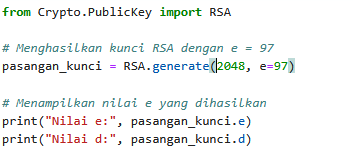
\includegraphics[width=0.85\textwidth]{../../images/python/page_040_img_01.png}

\end{document}
